\documentclass[12pt]{article}
\usepackage{graphicx}
\usepackage{caption}
\usepackage[margin=1in]{geometry}
\usepackage{float}
\usepackage[export]{adjustbox}
\usepackage{amsmath}
\usepackage{epstopdf}
\usepackage{subcaption}
\usepackage{amssymb}
\usepackage{listings}
\usepackage{scrextend}

\lstset{basicstyle=\ttfamily} 

\begin{document}

\title{\ \\ \ \\ \ \\ \ \\ \ \\Hybrid Stability Automata\\ \ \\ \ \\ \begin{Large} User Manual \\ \ \\
\end{Large}}
\date{July 2017}
\author{Peter Uth}
\maketitle

\newpage

\tableofcontents

\newpage


\section{Overview}
A hybrid stability automaton (HSA) is a method of modeling a dynamical system as a series of control modes and switches that are dependent on stability criteria. By employing numerical continuation to access fundamental stability properties and determine stable and unstable operating conditions, HSA can provide valuable information for safety analyses of physical systems. Refer to \cite{Uth_Thesis2017, Uth_Scitech2018} for the complete details on HSA.

This document provides details on how to generate HSA using the MATLAB tools developed for this work. HSA can be created for the following types of systems:

\begin{itemize}
\item One-dimensional, one-parameter (1D1P)
\item One-dimensional, multi-parameter (1DMP)
\item Multi-dimensional, one-parameter (MD1P)
\item Multi-dimensional, multi-parameter (MDMP)
\end{itemize}

\noindent Note that currently the multi-dimensional tools only work for two-dimensional systems. However, these tools are designed to accept higher-dimensional systems given some modifications planned as future work.


\section{Installation}

\subsection{Dependencies}
\label{dependencies}
Dependencies for the HSA tools are listed below. 

\begin{itemize}
\item MATLAB
	\begin{itemize}
	\item symbolic math toolbox
	\end{itemize}
\item Continuation-based System Analysis tool (COSY)
	\begin{itemize}
	\item \texttt{cosy.m}
	\item \texttt{cm\_pseudo\_arclength.m}
	\item \texttt{cm\_solution.m}
	\end{itemize}
\item GraphViz \cite{Gansner2000, Gansner2006, Ellson}
\item dot2tex (optional) \cite{Fauske}
	\begin{itemize}
	\item Python 2.6 or 2.7
	\item pyparsing
	\item preview-latex
	\item PGF/TikZ
	\end{itemize}
\end{itemize}

\subsection{Installation Process}
With the dependencies from Section \ref{dependencies} installed, place the three COSY files into the working directory or add the containing folder to the MATLAB path. The folder containing the GraphViz file \texttt{dot.exe} must be added to the system's environmental variables. Note that the HSA code has only been tested using the Windows operating system.


\section{One-Dimensional Systems}
HSA for one-dimensional systems (i.e. systems with one state) can be generated using the \texttt{hsa1D.m} file. For one-parameter systems (i.e. 1D1P), the \texttt{hsa1D} function can be called directly using the results from a COSY continuation process. For multi-parameter systems (i.e. 1DMP), \texttt{dataMP.m} must first be called and the resulting data is then passed to \texttt{hsa1D}. Details on these HSA tools and examples for 1D1P and 1DMP systems are presented in the following sections.


\subsection{hsa1D.m}
The \texttt{hsa1D} function creates HSA for 1D systems. 

\subsubsection{Inputs}
\begin{itemize}
\item \textbf{label} - Name of the file used for labeling outputs. Input as a string.

\item \textbf{F} - System equation(s). Input as a function handle. Use data output of \texttt{dataMP} for multi-parameter systems.

\item \textbf{B} - Solution branch data resulting from a COSY continuation analysis. Use data output from \texttt{dataMP} for multi-parameter systems.

\item \textbf{BP} - Solution branch point data resulting from a COSY continuation analysis. Use data output from \texttt{dataMP} for multi-parameter systems.

\item \textbf{P} - Parameter type selection:
	\begin{itemize}
	\item For fixed-$p$ case, input as the numerical $p$-value to be analyzed.
	\item For general case, input as empty (i.e. \texttt{[]}).
	\end{itemize}

\item \textbf{opt} - User options, if desired. Input as struct with any or all of the following fields:
	\begin{itemize}
	\item \textbf{dot2tex} - Enables LaTeX-style formatting in the visualization output. Input as a string (e.g. \texttt{opt.dot2tex = `on'}). Alternatively, a string input alone can be used if this is the only desired option (e.g. pass `dot2tex' to \texttt{hsa1D} instead of \texttt{opt}).
	\item \textbf{texlab} - Replaces states and parameters, default $x$ and $p$, with other symbols for visualization purposes. Input as a cell with a replacement defined within each row (e.g. \texttt{opt.texlab = \{`x' `\textbackslash gamma ';`p\_1' `\textbackslash alpha '\}} will show $x$ as $\gamma$ and $p_1$ as $\alpha$). Requires dot2tex. A blank space should be entered at the end of a LaTeX symbol designation for proper formatting. A cell input alone can be used if this is the only desired option.
	\item \textbf{ztol} - Change zero tolerance. Default is \texttt{opt.ztol = 0.00001}. 
	\item \textbf{PD} - Parameter designation matrix, used only for multi-parameter systems. An array input alone can be used if this is the only desired option. See \texttt{dataMP.m} description below for more detail. 
	\end{itemize}
\end{itemize}

\subsubsection{Outputs}
\begin{itemize}
\item Stability data for all modes as a struct.
\item HSA visualization as a PNG file. If dot2tex is enabled, a PDF is also created.
\item Executable function m-file containing the dynamical equations with stability information. Stability behavior is displayed in the command window when accessed (i.e. the value towards which the system converges or whether the system diverges depending on the current state).
\end{itemize}


\subsection{dataMP.m}
The \texttt{dataMP} function automatically runs the COSY continuation process for each parameter designation defined by the user. The output data can then be passed to the \texttt{hsa1D} function to produce a multi-parameter HSA.

\subsubsection{Inputs}
\begin{itemize}
\item \textbf{f} - System equation. Input as a function handle.

\item \textbf{PD} - Parameter designation matrix. Each row initiates a COSY continuation analysis on subset dynamics created using the designations within each column (column index = parameter number). Each row must have one NaN designation to identify the parameter activated for continuation.

\item \textbf{x0} - Initial state conditions for COSY. Input as column array where the number of elements is the same as the number of rows in the parameter designation matrix.

\item \textbf{p0} - Initial conditions of the active parameter for COSY. Input as column array where the number of elements is the same as the number of rows in the parameter designation matrix.

\item \textbf{plim} - Parameter limits for the COSY processes. Input as two-column array where the number of rows is the same as the number of rows in the parameter designation matrix. First column contains the lower limit, second column contains the upper limit.

\end{itemize}

\subsubsection{Outputs}

\begin{itemize}
\item \textbf{F} - Function cell. First entry is the original dynamics, subsequent entries are the subset dynamics as defined by the parameter designation matrix.

\item \textbf{B} - COSY output solution branch data for all subset analyses.

\item \textbf{BP} - COSY output solution branch point data for all subset analyses.
\end{itemize}


\subsection{One-Parameter Examples}

\subsubsection{Saddle Node Bifurcation, Fixed-$p$}
\label{snhsa}
Code to create an HSA for the prototypical saddle node bifurcation system, $\dot{x}=p+x^2$, is shown below.

\begin{addmargin}[0.5in]{1em}
\begin{lstlisting}
F = @(x,u,p) p+x^2;  
x0 = -1; 
p0 = -1;
c = cosy(F,1,0,1);
c.p_min = -1;              
c.p_max = 1;
[B,BP] = c.trace_solution_branches(x0,[],p0);
mode = hsa1D(`SN_fp',F,B,BP,-0.5);
\end{lstlisting}
\end{addmargin}

\noindent Lines 1-7 identify the function handle, establish COSY settings, and run COSY to obtain the solution data. In line 8, this data is then passed to the \texttt{hsa1D} function. Also in line 8, the label \texttt{SN\_fp} and the fixed-$p$ value -0.5 are input to the \texttt{hsa1D} function. Note that no options were selected for this process, so \texttt{P} is the last input into \texttt{hsa1D}. Figure \ref{SN_fp} shows the resulting output visualization. 

\begin{figure}[H]
\begin{center}
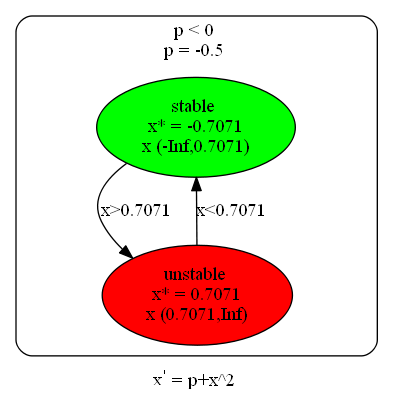
\includegraphics[width=2.5in]{SN_fp.png}
\caption{Hybrid stability automaton for a saddle node bifurcation, fixed-$p$ case.}
\label{SN_fp}
\end{center}
\end{figure}

\subsubsection{Saddle Node Bifurcation, General Case}
\noindent To produce the general case automaton shown in Figure \ref{SN_gen}, line 8 from Section \ref{snhsa} is replaced with:

\begin{addmargin}[0.5in]{1em}
\begin{lstlisting}
mode = hsa1D(`SN_gen',F,B,BP,[]);
\end{lstlisting}
\end{addmargin}

\begin{figure}[H]
\begin{center}
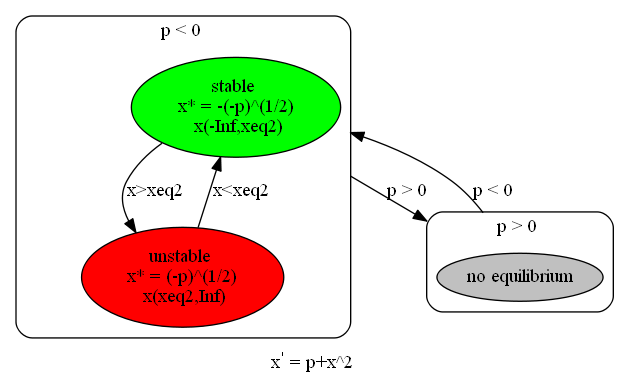
\includegraphics[width=4in]{SN_gen.png}
\caption{Hybrid stability automaton for a saddle node bifurcation, general case.}
\label{SN_gen}
\end{center}
\end{figure}

\noindent Figure \ref{SN_gentex} shows the general saddle node HSA with the dot2tex option enabled using the function call:

\begin{addmargin}[0.5in]{1em}
\begin{lstlisting}
mode = hsa1D(`SN_gen',F,B,BP,[],`dot2tex');
\end{lstlisting}
\end{addmargin}

\begin{figure}[H]
\begin{center}
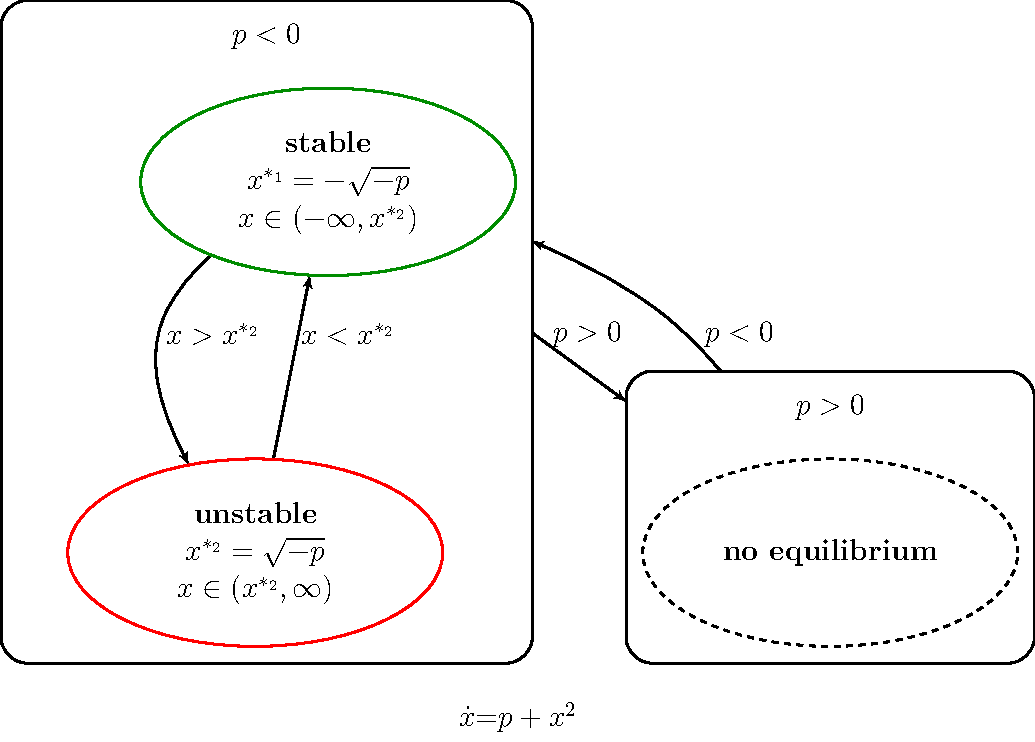
\includegraphics[width=4in]{SN_gentex.pdf}
\caption{Hybrid stability automaton for a saddle node bifurcation with dot2tex enabled, general case.}
\label{SN_gentex}
\end{center}
\end{figure}


\subsection{Multi-Parameter Examples}

\subsubsection{General Case}
\label{ODMP}
Consider the 1DMP system $\dot{x}=p_1+p_2x+p_3x^2-p_4x^3$ with the parameter designations

\begin{equation}
PD=\begin{bmatrix}
    NaN & 0 & 0 & 1\\
    0 & NaN & 0 & 1\\
    NaN & 0 & 1 & 0 
\end{bmatrix},
\end{equation}
which instructs the HSA tools to vary $p_1$ for cases 1 and 3, vary $p_2$ for case 2, and hold the other parameters as constants (0 or 1 in this example, but any constant values can be used). The following code can be used to create this system's HSA.

\begin{addmargin}[0.5in]{1em}
\begin{lstlisting}
f = @(x,u,p) p(1)+p(2)*x+p(3)*x^2-p(4)*x^3;
PD = [ NaN 0 0 1 ; 0 NaN 0 1 ; NaN 0 1 0 ];
x0 = [-1;-1;-1]; 
p0 = [-1;-1;-1];
plim = [-1 1;-1 1;-1 1];
[F,B,BP] = dataMP(f,PD,x0,p0,plim);
mode = hsa1D(`ODMP_gen',F,B,BP,[],PD);
\end{lstlisting}
\end{addmargin}

\noindent Lines 1-5 set up the problem and establish settings for the continuation process. Line 6 calls the \texttt{dataMP} function to create the continuation results for the three subset dynamics. Line 7 takes these results and produces the HSA for the general case. Figure \ref{ODMP_gen} shows the HSA.

\begin{figure}[H]
\begin{center}
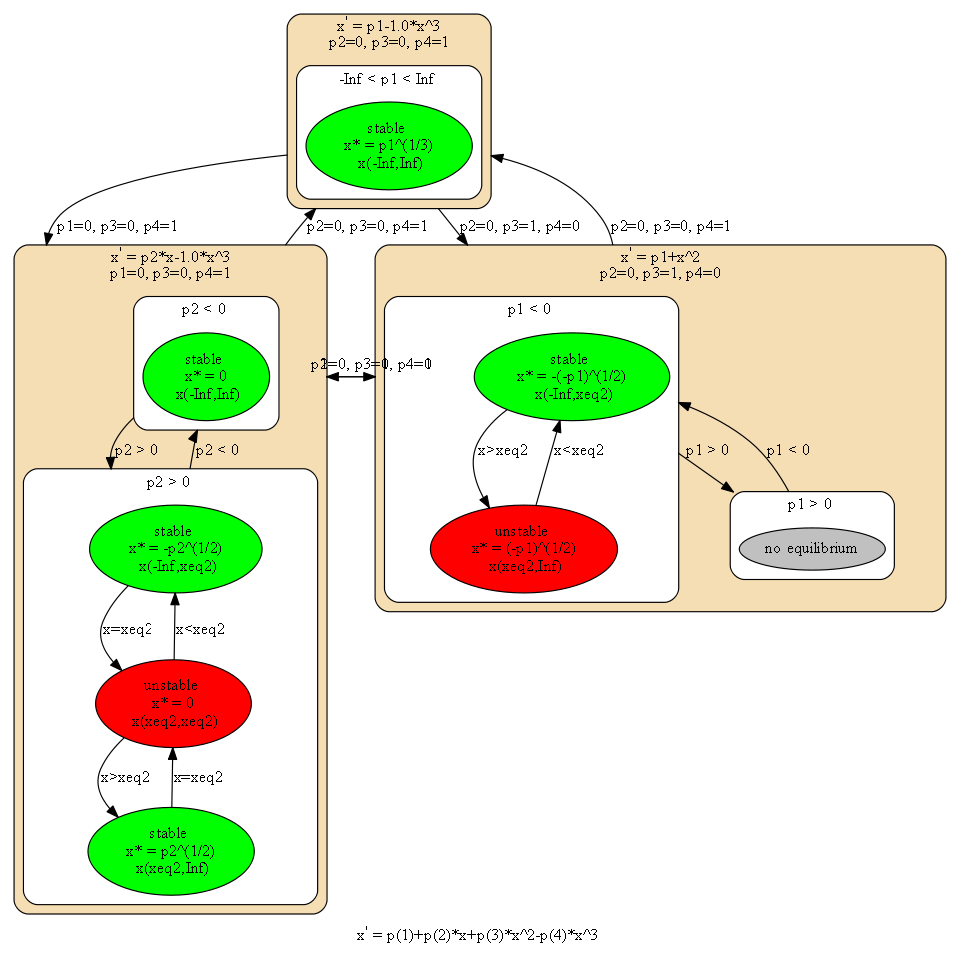
\includegraphics[width=4in]{ODMP_gen.png}
\caption{Hybrid stability automaton for a multi-parameter system, general case.}
\label{ODMP_gen}
\end{center}
\end{figure}


\subsubsection{Fixed-$p$ Case}
To produce a fixed-$p$ automaton of the system from Section \ref{ODMP} with $p=0.5$, dot2tex enabled, and states/parameters replaced with symbols in the visualization, line 7 can be replaced with the following lines:

\begin{addmargin}[0.5in]{1em}
\begin{lstlisting}
opt.PD = PD;
opt.dot2tex = `on';
opt.texlab = {`x' `\gamma';`p_1' `\alpha';
		`p_2' `v';`p_3' `h';`p_4' `\rho'};
mode = hsa1D(`ODMP_fp',F,B,BP,0.5,opt);
\end{lstlisting}
\end{addmargin}

\noindent The resulting HSA is shown in Figure \ref{ODMP_fp}.

\begin{figure}[H]
\begin{center}
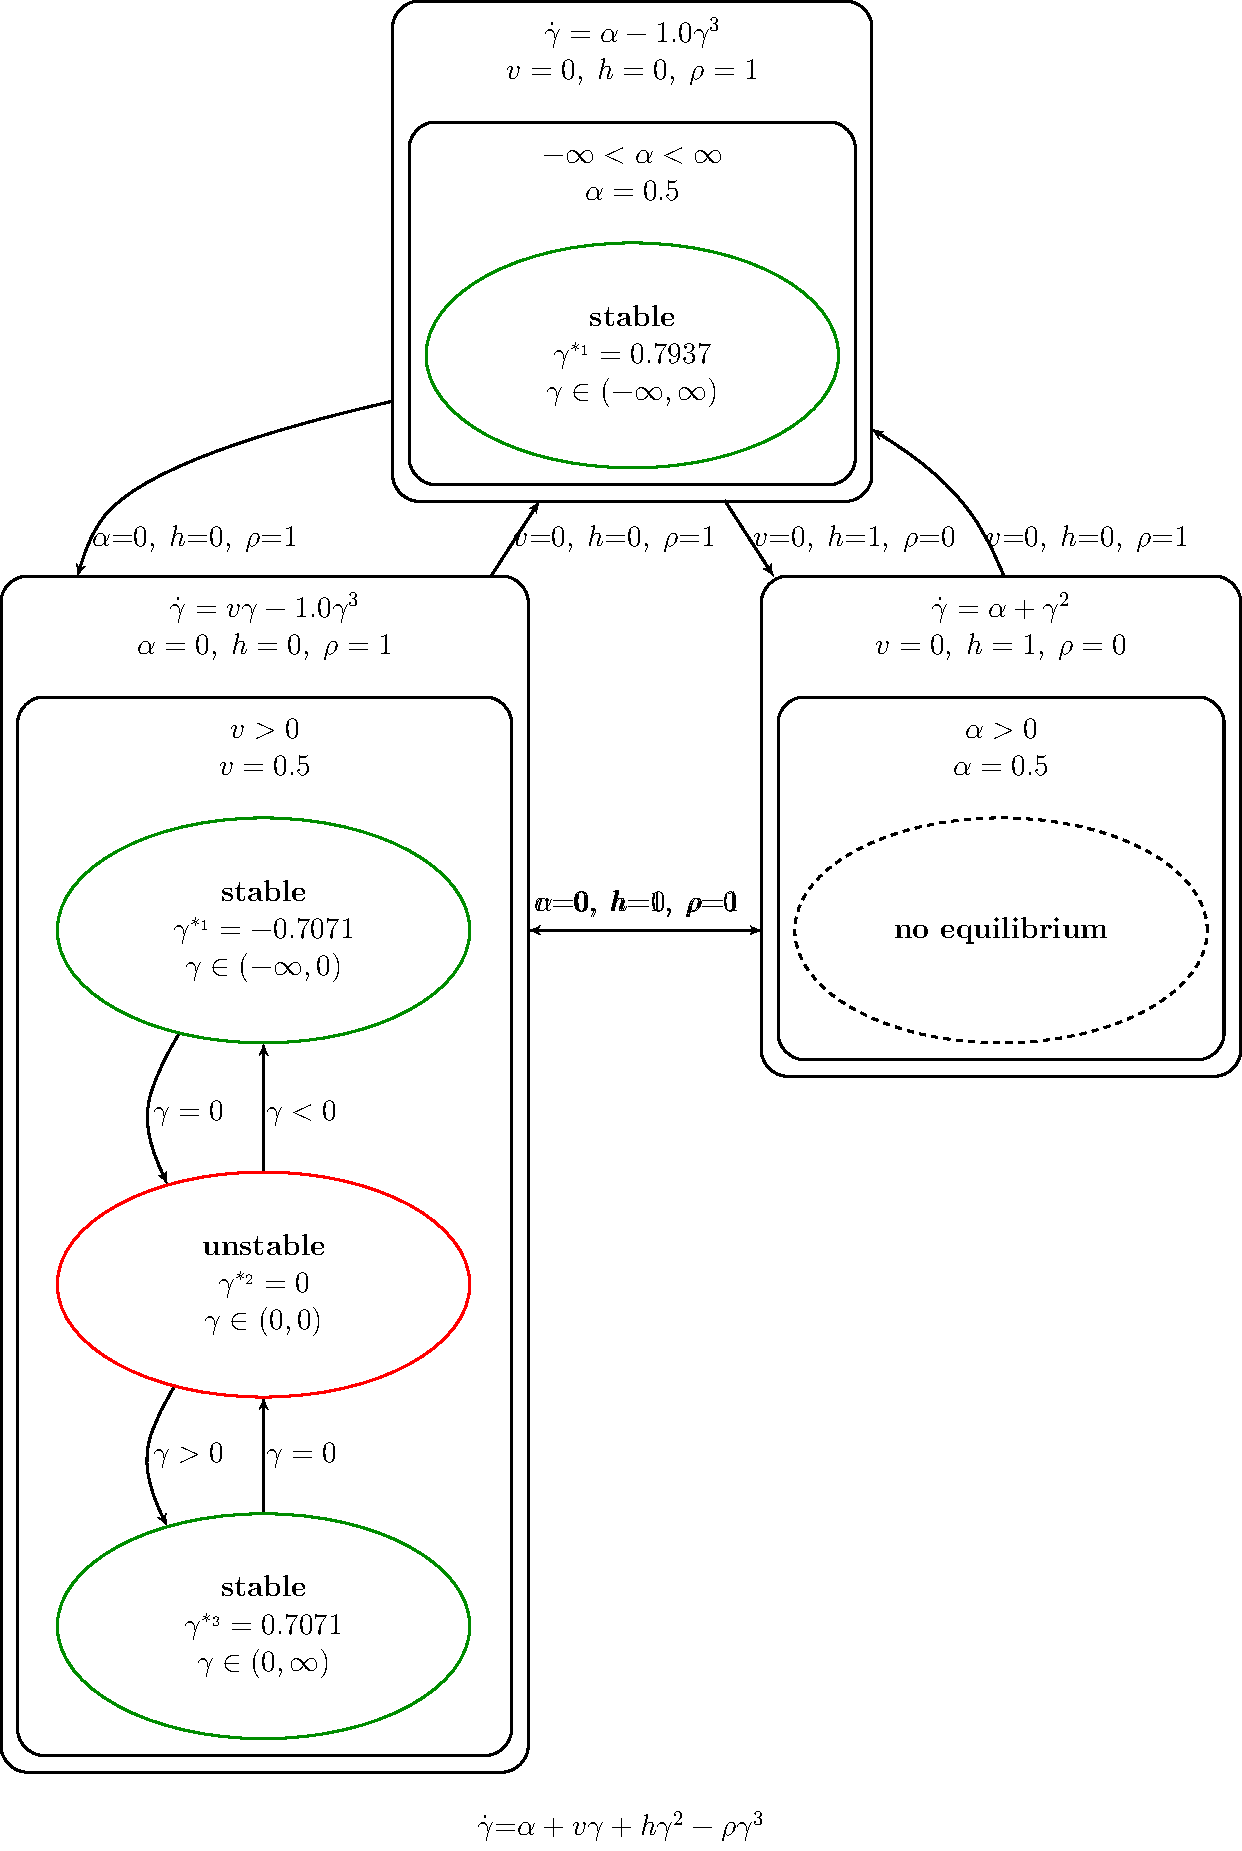
\includegraphics[width=4in]{ODMP_fpTexR.pdf}
\caption{Hybrid stability automaton for a multi-parameter system, fixed-$p$ case.}
\label{ODMP_fp}
\end{center}
\end{figure}


\section{Multi-Dimensional Systems}
HSA for multi-dimensional systems (i.e. systems with more than one state) can be generated using the \texttt{hsaMD.m} file. Similar to the 1D tools, the \texttt{hsaMD} function can be called directly for one-parameter systems (i.e. MD1P). For multi-parameter systems (i.e. MDMP), \texttt{dataMP} must first be called and the resulting data is then passed to \texttt{hsaMD}. A separate basin of attraction identification step can be applied using \texttt{basinMD.m} if desired. Details on the multi-dimensional tools and examples for MD1P and MDMP systems are presented in the following sections.


\subsection{hsaMD.m}
The \texttt{hsaMD} function creates HSA for MD systems. The inputs and outputs of this function are the same as \texttt{hsa1D} except for the following differences:

\begin{itemize}
\item The input function state must have multiple elements (e.g. \texttt{x(1)} and \texttt{x(2)}).
\item The outputs do not explicitly define the basins of attraction. In the visualization, the basins are generically defined. In the executable file, the stability behavior is not displayed when accessed unless data from the \texttt{basinMD} function is available.
\end{itemize}


\subsection{basinMD.m}
Unlike for 1D systems, the basins of attraction for stable equilibria in MD systems cannot be automatically deduced from the continuation data output. The \texttt{basinMD} function can be used to approximate a basin using different methods. Currently, only repeated simulation methods are available, but the \texttt{basinMD.m} file is structured to allow the addition of new method selections. Basin identification only works for fixed-$p$ cases.


\subsubsection{Inputs}
\begin{itemize}
\item \textbf{mode} - Output mode data from the \texttt{hsaMD} function.

\item \textbf{type} - Basin of attraction identification method. Input as string. Currently available:
	\begin{itemize}
	\item \textbf{Simulation} - Repeated simulation using fixed-step sampling.
	\item \textbf{MonteCarlo} - Repeated simulation using random sampling.
	\end{itemize}

\item \textbf{xlimit} - The desired state limits for the basin identification process. Input as array where the row index is the state number, column 1 contains the lower limits, and column 2 contains the upper limits.

\item \textbf{segs} - Number of samples. For the \texttt{Simulation} type, this is the number of samples in each dimension (e.g. \texttt{segs=10} will yield 100 samples in a 2D system). For the \texttt{MonteCarlo} type, this is the total number of random samples.

\item \textbf{tspan} - Time span for the simulations. Input as row array where the first element is the start time and the second element is the end time. 
\end{itemize}

\subsubsection{Outputs}
\begin{itemize}
\item Basin of attraction approximations for all stable basins as a struct.
\item Visualizations of the basin approximations.
\end{itemize}


\subsection{One-Parameter Example}
Code to create an HSA for the 2D dynamical system, 

\begin{equation}
\begin{bmatrix}
\dot{x_1} \\ \dot{x_2}
\end{bmatrix}
=
\begin{bmatrix}
-px_2-x_1^3 \\ -x_2^2-x_1
\end{bmatrix},
\end{equation}
is shown below. 

\begin{addmargin}[0.5in]{1em}
\begin{lstlisting}
F = @(x,u,p) [ -p*x(2)-x(1)^3 ; -x(2)^2-x(1) ];
x0 = [-1;-1]; 
p0 = -1;
c = cosy(F,2,0,1);
c.p_min = -10; 
c.p_max = 10;
c.x_max = [10;10]; 
c.x_min = [-10;-10];
c.cm.max_steps = 15000;
[B,BP] = c.trace_solution_branches(x0,[],p0);
mode = hsaMD(`MD1P_gen',F,B,BP,[],`dot2tex');
\end{lstlisting}
\end{addmargin}

\noindent The resulting HSA is shown in Figure \ref{MD1P_gen}.

\begin{figure}[H]
\begin{center}
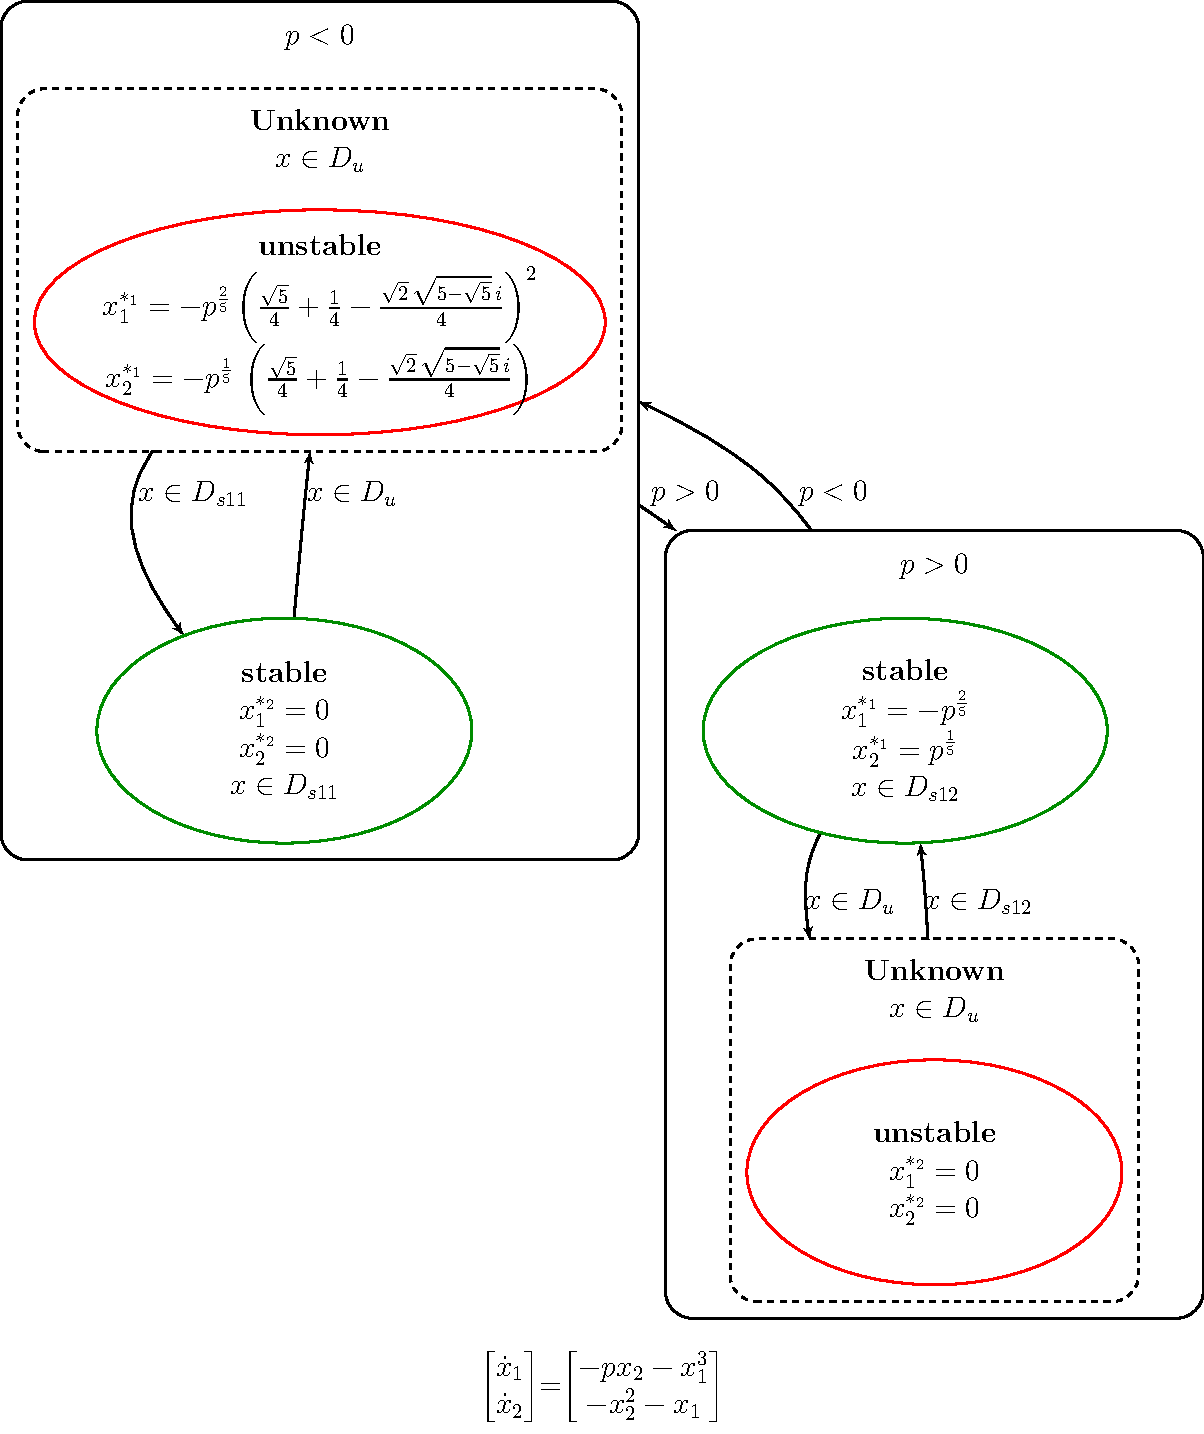
\includegraphics[width=4.5in]{MD1P_genTex.pdf}
\caption{Hybrid stability automaton for a 2D, one-parameter system, general case.}
\label{MD1P_gen}
\end{center}
\end{figure}


\subsection{Multi-Parameter Example}
Consider the MDMP system,

\begin{equation}
\begin{bmatrix} \dot{x_1} \\ \dot{x_2}
\end{bmatrix}
=
\begin{bmatrix}
-p_1x_2+p_2x_1-x_1^3 \\
-p_3\left(x_2^2+x_1\right)+p_2x_1-p_4x_1^2
\end{bmatrix},
\end{equation}
with the parameter designation matrix, 

\begin{equation}
PD=\begin{bmatrix}
    NaN & 0 & 1 & 0\\
    1 & NaN & 0 & 1
\end{bmatrix}.
\end{equation}
The following code can be used to create a fixed-$p$ HSA for this system with $p=-0.5$.

\begin{addmargin}[0.5in]{1em}
\begin{lstlisting}
f = @(x,u,p) [ -p(1)*x(2)+p(2)*x(1)-x(1)^3 ;
	-p(3)*(x(2)^2+x(1))+p(2)*x(1)-p(4)*x(1)^2 ];
PD = [ NaN 0 1 0 ; 1 NaN 0 1 ];
x0 = [0 0;0 0];
p0 = [-1;-1];
plim = [-10 10;-10 10];
[F,B,BP] = dataMP(f,PD,x0,p0,plim);  
opt.PD = PD;
opt.dot2tex = `on';
mode = hsaMD(`MDMP_fp',F,B,BP,-0.5,opt);   
\end{lstlisting}
\end{addmargin}

\noindent The resulting HSA is shown in Figure \ref{MDMP_fp}.

\begin{figure}[H]
\begin{center}
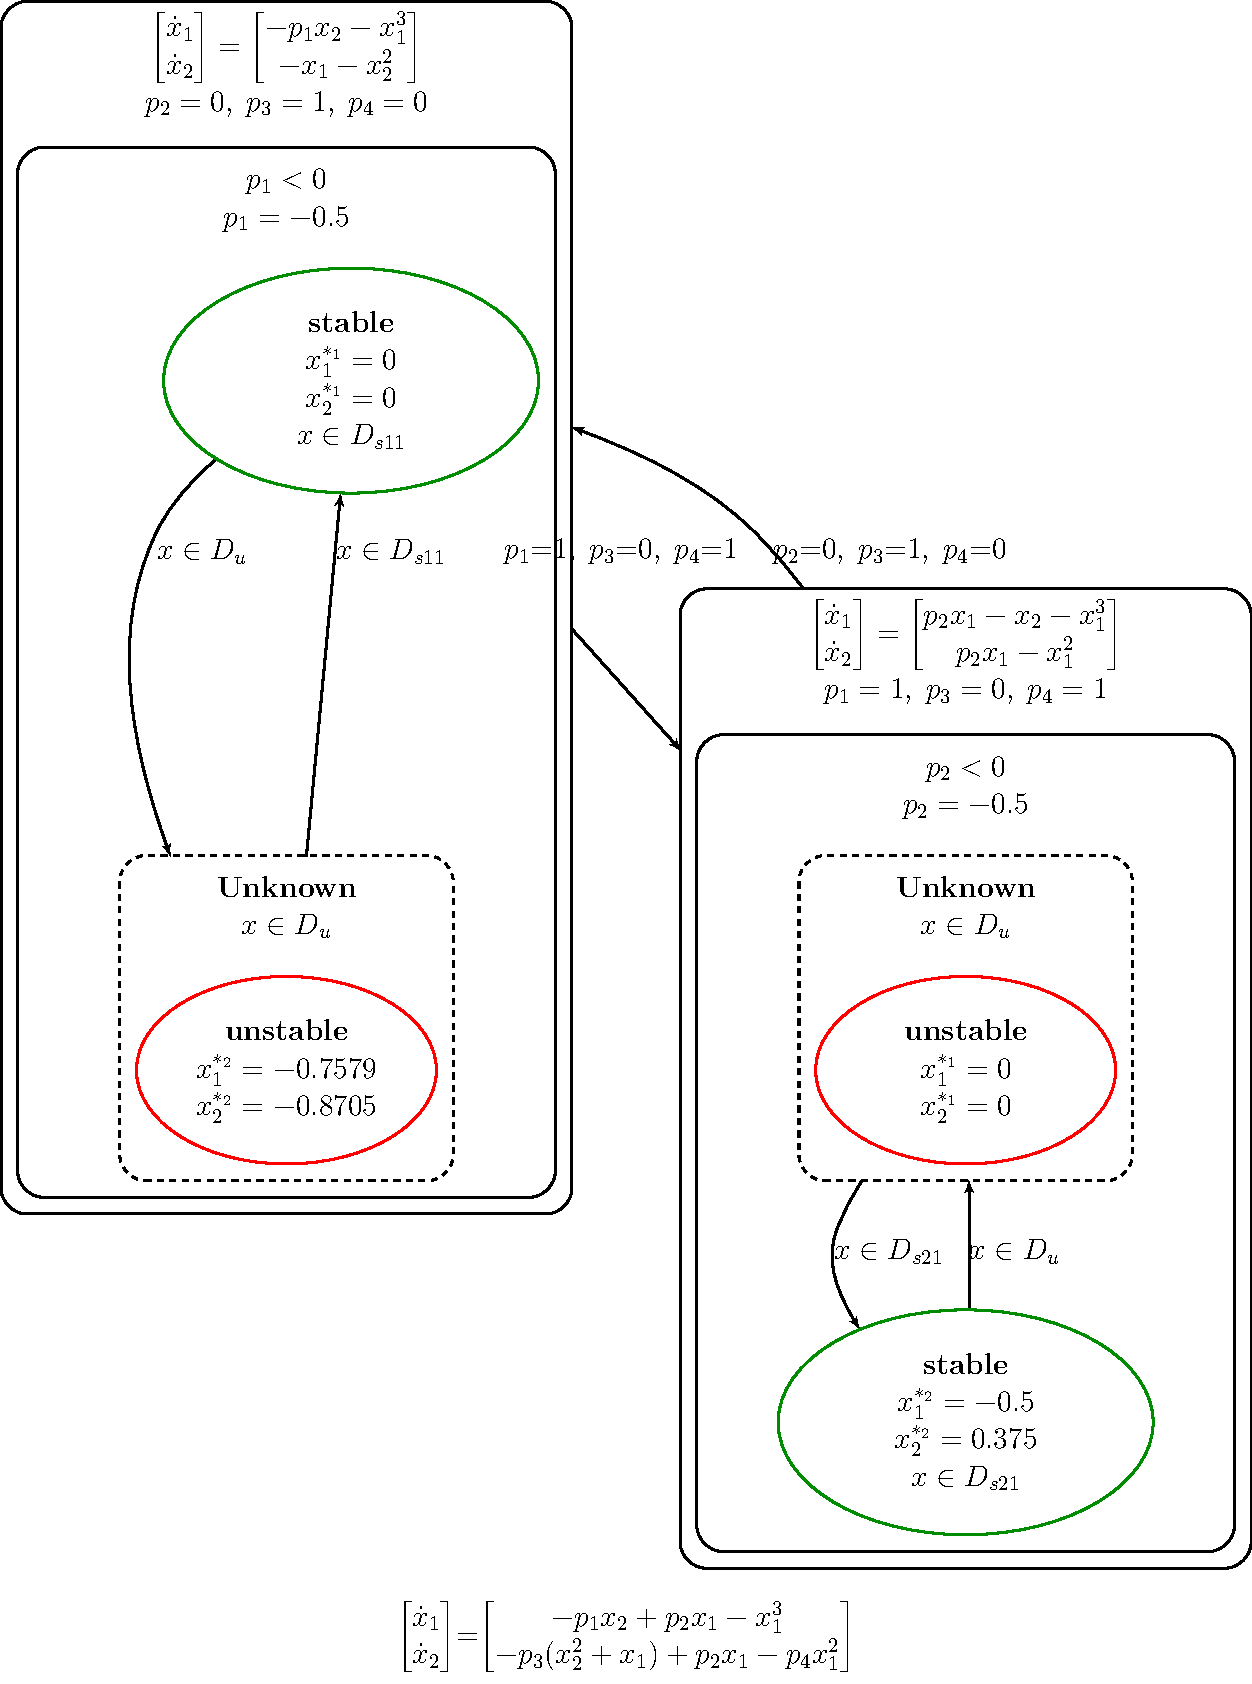
\includegraphics[width=4.5in]{MDMP_fpTex.pdf}
\caption{Hybrid stability automaton for a 2D, multi-parameter system, fixed-$p$ case.}
\label{MDMP_fp}
\end{center}
\end{figure}

The \texttt{basinMD} function can be used to obtain approximations for the generically defined $D_{s11}$ and $D_{s21}$ basins of attraction. The following code establishes settings and applies the \texttt{basinMD} function with the \texttt{Simulation} method selected.

\begin{addmargin}[0.5in]{1em}
\begin{lstlisting}
xlimit = [-3 3;-3 3];
tspan = [0 20];
segs = 10; 
basin = basinMD(mode,`Simulation',xlimit,segs,tspan);
\end{lstlisting}
\end{addmargin}

\noindent The visualizations for the resulting basin approximations are shown in Figures \ref{Ds11_basin} and \ref{Ds21_basin}.

\begin{figure}[H]
\begin{center}
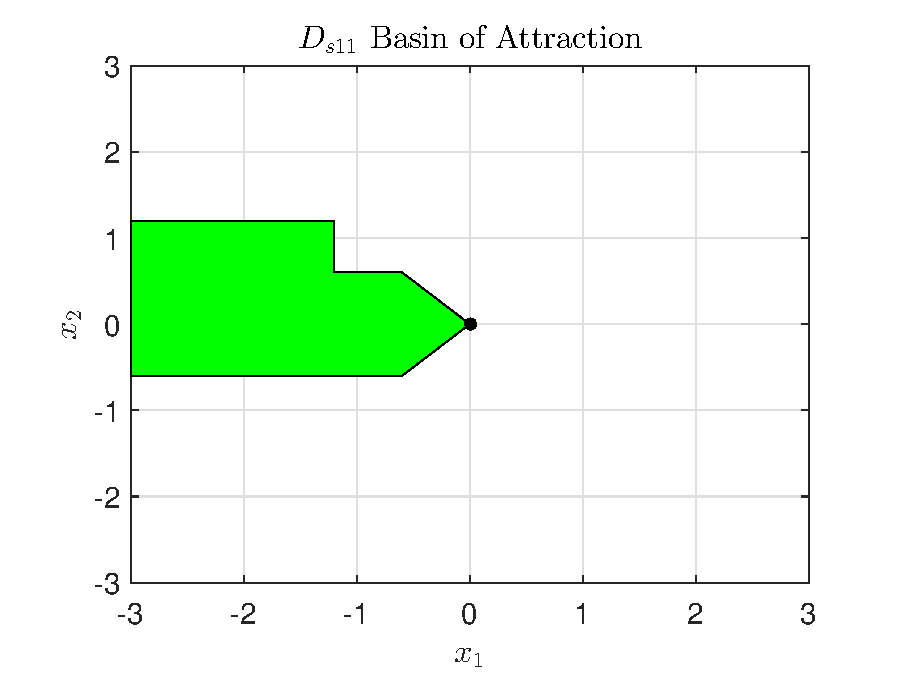
\includegraphics[width=4in]{Ds11_basin.eps}
\caption{Basin of attraction approximation for $D_{s11}$.}
\label{Ds11_basin}
\end{center}
\end{figure}

\begin{figure}[H]
\begin{center}
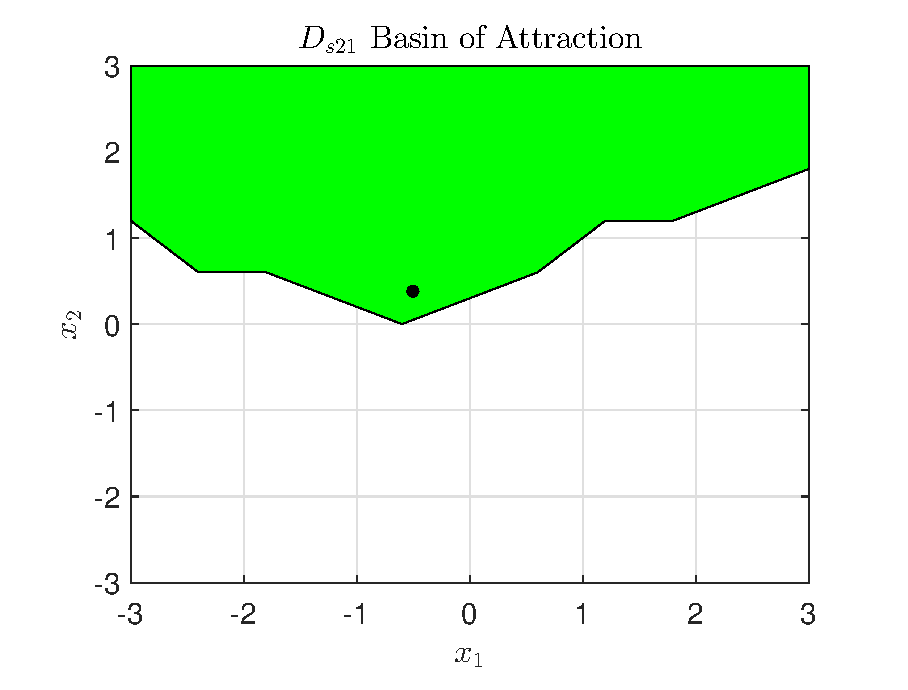
\includegraphics[width=4in]{Ds21_basin.eps}
\caption{Basin of attraction approximation for $D_{s21}$.}
\label{Ds21_basin}
\end{center}
\end{figure}


%========== Bibliography =======================
%\nocite{*}  
\bibliographystyle{aiaa}
\bibliography{HSA_User_Manual}

%\bibliographystyle{unsrt}
%\bibliography{AFRL_UW_Report}

\end{document}
